\subsection{Decision Tree}

We have created decision trees using the four different kinds of input as described in (??TODO Reference). The output of these decision trees can be seen in Figure \ref{decisionTrees}.

\begin{figure}
	\begin{subfigure}[b]{0.5\textwidth}
	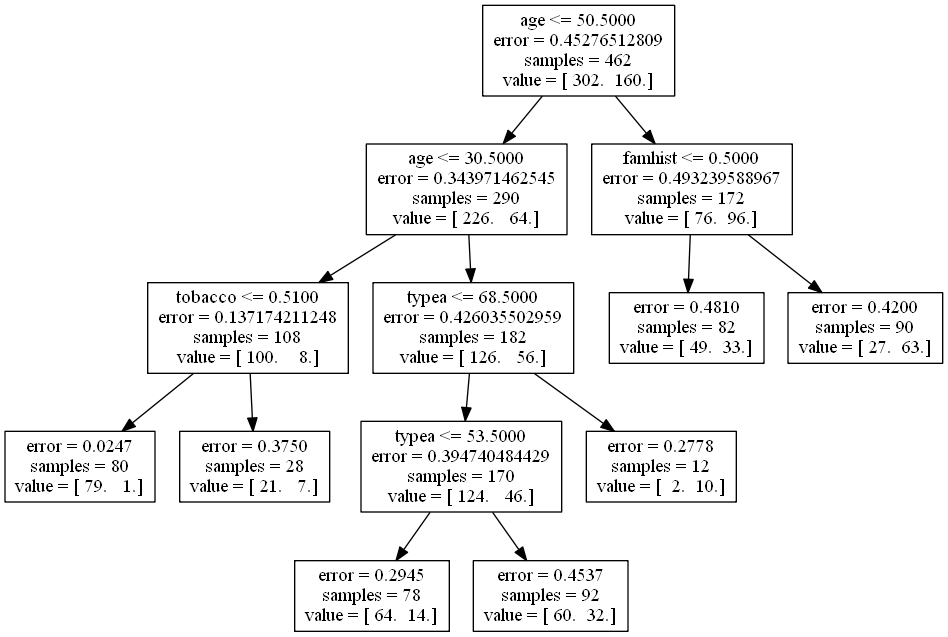
\includegraphics[scale=0.2]{pictures/Decision_Tree_X.png}
	\caption{Looking at all attributes.}
	\label{decisionTreeX}
	\end{subfigure}
	\begin{subfigure}[b]{0.5\textwidth}
	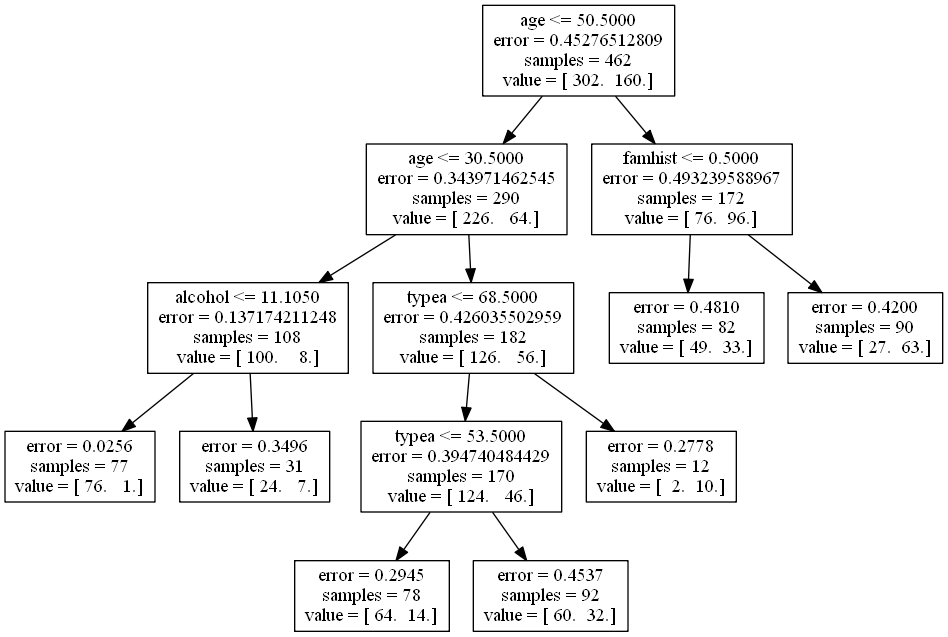
\includegraphics[scale=0.2]{pictures/Decision_Tree_Xad.png}	
	\caption{Looking at attributes selected by forward selection.}
	\label{decisionTreeXad}
	\end{subfigure}

	\begin{subfigure}[b]{0.5\textwidth}
	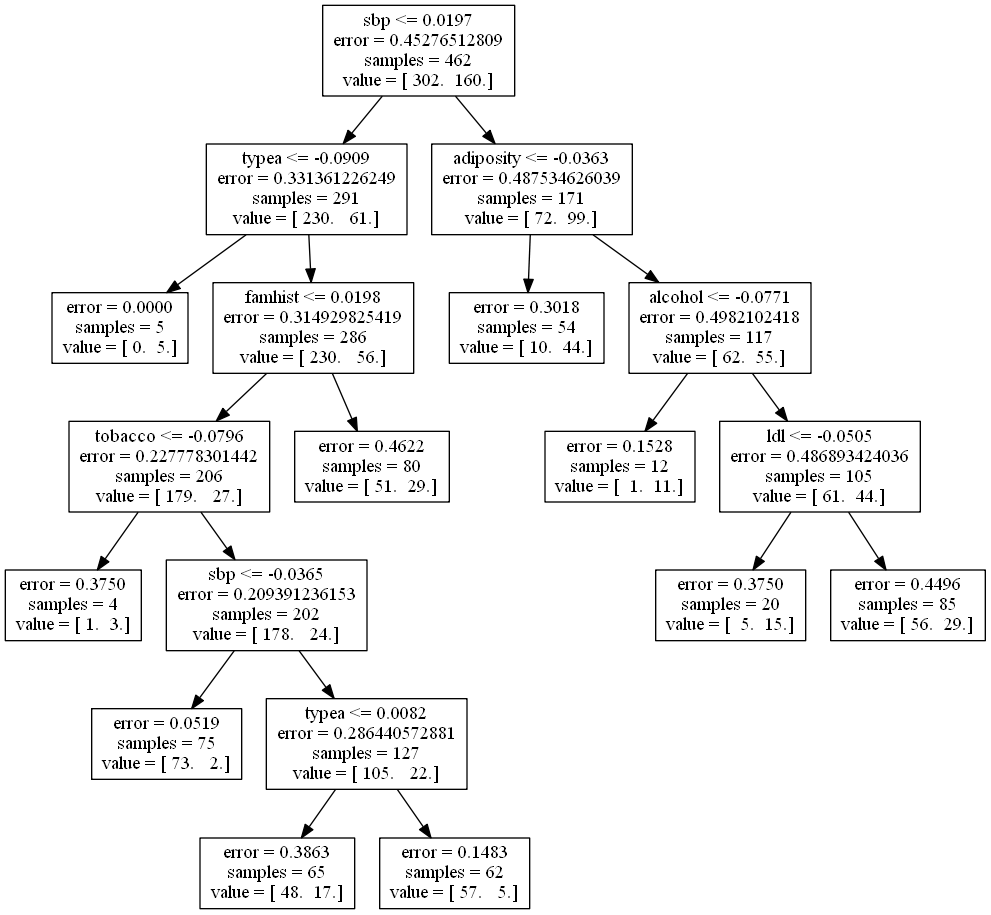
\includegraphics[scale=0.2]{pictures/Decision_Tree_XPC.png}
	\caption{Looking at all principal components.}
	\label{decisionTreeXPA}
	\end{subfigure}
	\begin{subfigure}[b]{0.5\textwidth}
	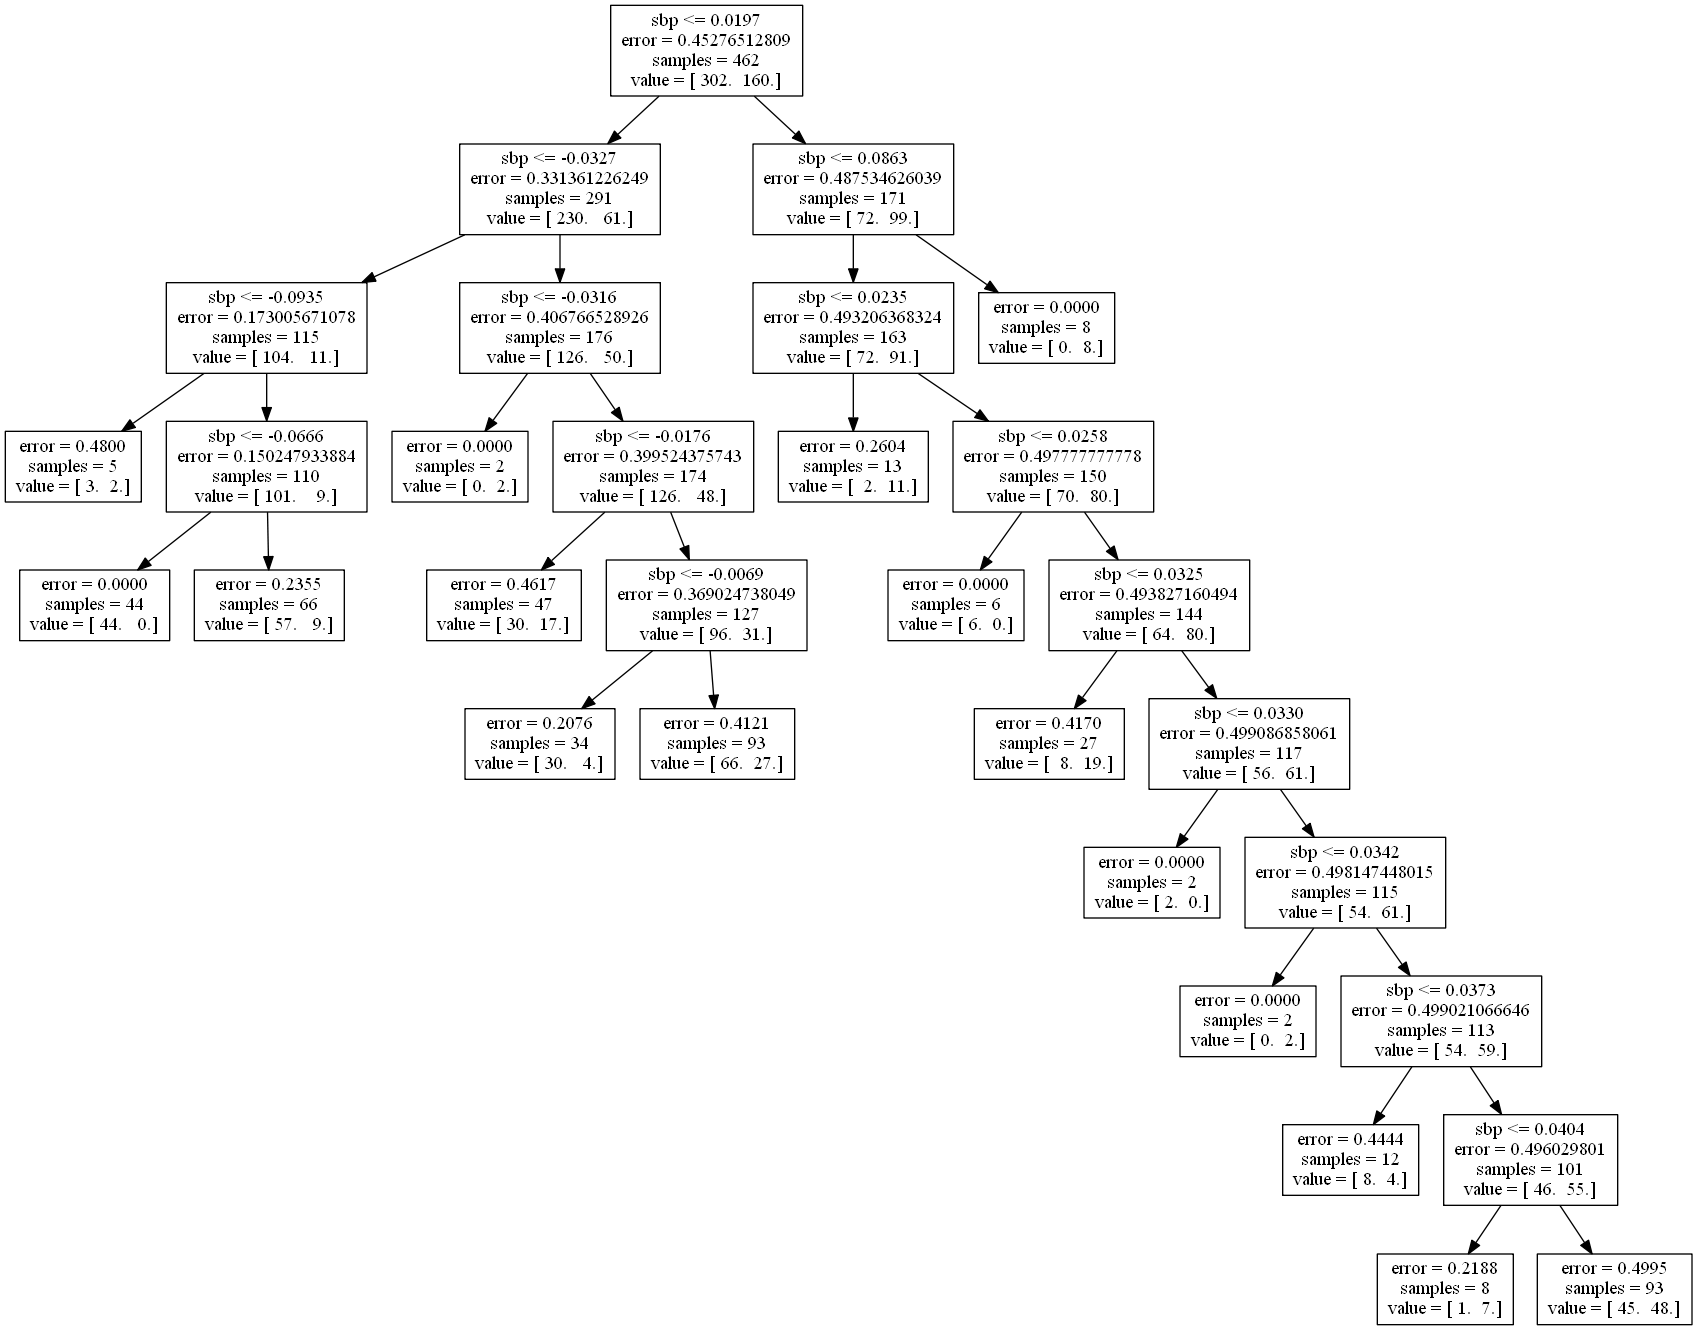
\includegraphics[scale=0.2]{pictures/Decision_Tree_X2PC.png}
	\caption{Looking at two most important principal components.}
	\label{decisionTreeX2PA}
	\end{subfigure}
\caption{This figure shows decision trees calculated based on different inputs.}
\label{decisionTrees}
\end{figure}

Now one can use such decision trees to classify data objects, which is simply done by following branches of the tree, until one reaches a leaf, which then either represent people with negative or positive CHD.

Therefore one can go through each data object, and compare how it will be classified according to the decision trees and which value it truly has. This way we have calculated the misclassification error, which can be seen in Figure \ref{decisionTreeErrorRate}

\begin{table}
\begin{longtable}{|l|l|}
Result from: & Mis-classification rate \\ \hline
Figure \ref{decisionTreeX} & 25,1\% \\ \hline 
Figure \ref{decisionTreeXad} & 25,1\% \\ \hline
Figure \ref{decisionTreeXPA} & 21,4\% \\ \hline
Figure \ref{decisionTreeX2PA} & 25,1\% \\ \hline
\end{longtable}
\caption{Mis-classification rates of decision trees.}
\label{decisionTreeErrorRate}
\end{table}

For making these decisions trees, we have used the whole data set as input. Furthermore, we have defined that the a node need to contain at least 100 objects in order to be split up. As we use the whole data set as input for the decision tree, and we also calculate the mis-classification rate according to how well the tree can classify objects from our data set, then by defining a very low lower bound for when to split up nodes, we can get a very high classification rate.
